\documentclass[parskip=full]{article}

% functionality
% formatting
\usepackage[utf8]{inputenc} % allow utf-8 input
\usepackage[T1]{fontenc} % use 8-bit T1 fonts  (allows for direct use of ö,ü,etc.)

% math typesetting
\usepackage{amsmath}
\usepackage{amssymb}
\usepackage{amsfonts}

% maths definitions, theorems, etc.
\usepackage{amsthm}

% color
\usepackage{color}
\usepackage{xcolor}

% layout
\usepackage{layout}
\usepackage{lipsum}

% cross-referencing and hyperlinks
\usepackage{hyperref}
\usepackage{url}
\usepackage{doi}

% figures
\usepackage{graphicx}
\usepackage{subfig}
\usepackage{wrapfig}

% tables
\usepackage{booktabs}
\usepackage{multirow}
\usepackage{caption} 
\usepackage{float}

% enumeration
\usepackage{enumitem}

% embedding pages
\usepackage{pdfpages}

% multi-line comments
\usepackage{comment}

% landscape orientation
\usepackage{rotating}
\usepackage{pdflscape}

% Gantt charts
\usepackage{pgfgantt}

% footnotes
\usepackage{footnote}

% code
\usepackage{listings}

% matrices and tables
\usepackage{nicematrix}
\usepackage{varwidth}
% \usepackage{tabularx} do not load package tabularx, instead use package nicematrix

% document structure
\setcounter{secnumdepth}{5} % enable numbered sub-sub-sections etc.

% custom header size
\usepackage{titlesec}

% custom titles
\usepackage{titling}

% customized references (make "Figure 1" a link, not just "1")
\usepackage[capitalise, nameinlink]{cleveref}

% customized frames around text etc.
\usepackage{mdframed}

% tikz
\usepackage{tikz}
\usetikzlibrary{fit}
\usetikzlibrary{calc,shadings,patterns}

% calligraphy
\usepackage{calligra}

% chemical formulas
\usepackage{chemformula}

% highlighting
\usepackage{soul} % to be used together with xcolor

% layout
% column layout
\usepackage{multicol}
\setlength{\columnsep}{0.75cm}

% paragraphs
\usepackage[skip=0.5\baselineskip]{parskip}

% geometry
\usepackage[
    margin = 3cm,
    top = 3cm,
    bottom = 3cm
]{geometry}

% header size
\titleformat*{\section}{\large\bfseries}%{\thesection.}{\hspace{0cm}}{}
\titleformat*{\subsection}{\normalsize\bfseries}%{\thesection.}{\hspace{0cm}}{}
\titleformat*{\subsubsection}{\normalsize\bfseries}
\titleformat*{\paragraph}{\normalsize\bfseries}
\titleformat*{\subparagraph}{\normalsize\bfseries}

% custom headers
\usepackage{fancyhdr}

% bibliography
\usepackage[
    backend=biber,
    style=ieee
]{biblatex}

% show DOI URL (https://doi.org/XXX.XXXXX.XXXX), instead of publisher URL (https://springer.com/XXXX)
% cf. https://tex.stackexchange.com/a/616241
\DeclareSourcemap{
  \maps[datatype = bibtex]{
    \map{
      \step[notfield = keywords, final]
      \step[fieldsource = doi, final]
      \step[fieldset = url, null]
    }
    \map{
      \step[fieldsource = keywords, notmatch = \regexp{\bprimary\b}, final]
      \step[fieldsource = doi, final]
      \step[fieldset = url, null]
    }
  }
}
\AtEveryBibitem{
    \clearfield{urlyear}
    \clearfield{urlmonth}
}
\addbibresource{bibliography.bib}

%% METADATA %%%%%%%%%%%%%%%%%%%%%%%%%%%%%%%%%%%%%%%%%%%%%%%%

\hypersetup{
    pdftitle={Methods},
    pdfauthor={Michael Weinold, Sergey Kolesnikov, Laura Diaz Anadon},
}

%% MAIN DOCUMENT %%%%%%%%%%%%%%%%%%%%%%%%%%%%%%%%%%%%%%%%%%%

\begin{document}

\setlength{\fboxsep}{10pt}
\fbox{
    \parbox{\textwidth}{
        \textit{\textsc{Methods Information}} for: \\
        \newline 
        M. Weinold$^{1,2,3}$, S. Kolesnikov$^3$, L.D. Anadon$^{3,4}$ \\
        "Rapid technological progress in white light-emitting diodes and its sources in innovation and technology spillovers" \textit{Nature Energy} (2023) \\
        \newline
        $^1$ Technology Assessment Group, Paul Scherrer Institute, Switzerland \\
        $^2$ ETH Zurich, Zurich, Switzerland \\
        $^3$ CEENRG, Dept. of Land Economy, University of Cambridge, UK \\
        $^4$ Belfer Center for Science and International Affairs, Harvard University, Cambridge MA, USA
    }
}

\section{Overview}
\label{sec:methods}

The evolution of LED device architecture and performance as well as the progress in understanding the underlying physical phenomena are well covered in the scholarly literature and patents. However, information provided in such sources is insufficient for our goals on at least three accounts: First, existing work focuses only on selected performance parameters or overall device efficiency, rather than on providing a comprehensive coverage of the whole device sub-efficiencies for a particular LED product or design. Scientific publications also do not always disclose the underlying device architecture or the features responsible for the gains in performance. Second, not all relevant innovations are patented \cite{Pakes_1980,Fontana_2013}. In the case of LED patents in particular, our interviews with industry experts suggest that the propensity to patent is the highest for knowledge related to macroscopic device architecture and chemical composition of phosphors, and the lowest for knowledge related to manufacturing process improvements and microscopic chip architecture that is difficult to reconstruct by reverse engineering. This means that relying only on patent literature would bias results by unduly emphasizing some focus areas and de-emphasizing others. Third, scientific publications and patents typically focus on experimental devices, rather than commercial products. While new LED features, designs and manufacturing methods reported in these sources can potentially result in significant performance gains or cost reductions, it is difficult to ascertain if these improvements have since been adopted in industry.  Furthermore, information on LED manufacturing cost and the effect of process improvements on the total cost is highly proprietary. Estimates are occasionally reported in the scientific literature and company publications, but these often do not disclose which parts of the manufacturing process are responsible for the largest contribution to the overall cost, or which improvements led to cost reductions.

To overcome the limitations of these different methods for understanding technological progress, in this study we rely on a multi-method approach to data collection and analysis, the details of which are provided in Section 2 of the Supplementary Information document. Specifically, we combine information obtained from a systematic review of the primary scientific literature, device datasheets, relevant patents, and industry publications (SI Section 2.1) with information gained from semi-structured interviews with experts from academia and industry (SI Section 2.2), bottom-up manufacturing cost modelling (SI Section 2.3), and our own computations of device sub-efficiencies (SI Section 2.4). We then use this information to track the historical progress in white LED technology over time across the three groups of metrics identified above in the 'Metrics' section and identify its sources in innovation and technology spillovers.

\section{Methodology}
\label{sec:costmodel}

This subsection provides the details for the main methods and data sources used in our mixed-methods research approach, including the systematic literature review, semi-structured interviews with eminent experts, manufacturing cost modelling, and performance metrics calculations.

\subsection{Systematic Literature Review}

We collected data on LED performance and characteristics in a systematic literature review that included scientific publications, patents, conference proceedings from the largest semiconductor and optoelectronics conferences, industry periodicals and roadmaps, as well as company presentations and reports. This review was structured around the three main goals: 1) tracking the evolution of LED technology over time as indicated by three groups of progress metrics introduced in the main article; 2) identifying individual innovations that contributed to this evolution and whether or not they could be spillovers, and quantifying their impact on device performance and manufacturing cost; and 3) determining whether these innovations had originated within the LED technology domain, or in a field of research or technology outside of solid-state lighting, making them a technology spillovers. 

Relevant sources for the review were found in an iterative search process that involved two components. The first was the search in specialized patent and publication databases as well as company websites. The second component was the analysis of backward citations in the identified sources, starting from the reviews mentioned in section Previous Literature in the main article and then iteratively repeating it for all newly identified sources, until no further relevant and significant new sources were found. We also relied on backward citations for the identification of technology spillovers, considering cited documents as indicators of knowledge origins of an innovation and analyzing whether those documents belonged to the LED technology domain or not.

\subsection{Semi-Structured Interviews}

To supplement our data collection efforts, verify our findings and identify additional spillovers, we conducted a series of elite semi-structured interviews with eleven eminent experts from academia, industry and the public research sector. Experts were selected based on their engagement in  different sub-fields of LED research and manufacturing, as well as the recommendations from other interviewed experts, in essence expanding the list of experts that emerged from the initial literature review. All interviews were conducted between November 2019 and April 2022 by means of video conferencing and lasted for about one hour. A summary of the background of interviewed experts is provided in \cref{tab:interviews}.

The primary, structured part of the interviews explored which innovations were deemed most relevant to the evolution of device performance, consumer experience and manufacturing cost of LED packages. Thereafter, interviewees were asked to consider the extent to which these innovations may have originated outside of their respective field of expertise and the LED industry more broadly—i.e., which of the innovations may be considered spillovers. The remainder of the interview was focused on learning about particular aspects of the manufacturing processes relevant to cost and performance modelling, the current state of industry, and the circumstances surrounding the innovations and spillovers identified in the first part of the interview. Specific quantitative data was also provided by experts, helping fine-tune the parameters of the manufacturing cost model (described in \cref{sec:costmodel}) and verify device performance data.

\begin{table}[H]
\small
    \centering
    \caption{Anonymized list of LED experts interviewed for this study. Abbreviations: sr. - senior}
    \vspace{5mm}
    \begin{tabular}{|l|l|l|l|l|}
    \hline
        \textit{\#} & \textit{Sector} & \textit{Role} & \textit{Country} & \textit{Expertise} \\ \hline
        1 & Academia & Sr. researcher & UK & Epitaxy \\ \hline
        2 & Industry & Consultant, former sr. researcher & USA & Device architecture \\ \hline
        3 & Industry & Consultant, former head of R\&D & Germany & Epitaxy \\ \hline
        4 & Academia & Professor & Austria & Phosphors \\ \hline
        5 & Industry & Consultant, former head of R\&D & USA & Device architecture \\ \hline
        6 & Consulting & Consultant, former sr. technical advisor & USA & Device architecture \\ \hline
        7 & Academia & Professor & Germany & Phosphors \\ \hline
        8 & Government & R\&D manager & USA & Device architecture \\ \hline
        9 & Consulting & Consultant & USA & Device applications \\ \hline
        10 & Academia & Professor & France & Device physics \\ \hline
        11 & Industry & Sr scientist, former head of R\&D & USA & Device architecture \\ \hline
        12 & Industry & Principal scientist & Germany & Phosphors \\ \hline
        13 & Industry & Former head of R\&D & USA & Phosphors \\ \hline
    \end{tabular}
    \label{tab:interviews}
\end{table}

\subsection{Performance Metrics Calculations}
\label{subsec:metrics}

The contribution of individual technology innovations and spillovers to the progress in overall device efficiency over time is estimated by index decomposition analysis. Mathematically, this involves breaking down a chosen performance indicator into its constituent components, each representing a specific factor that contributes to the change in the indicator \cite{Ang1997}. Specifically, we use the additive logarithmic mean Divisia index method I (LMDI-I), also known as the Additive Sato-Vartia indicator \cite{deBoer2019}. It was developed by Boyd in 1987 \cite{Boyd1987} on the basis of Divisia Index, a method in statistical economics \cite{Diewert1988}, and subsequently refined.

According to this method, for an overall device efficiency function $F$ that is the product of variables $a, b$ that represent sub-efficiencies, the contribution of the change in a single sub-efficiency variable $a$ between times $t=0$ and $t=T$ can be estimated as \cite{Ang2019}

\begin{align}
    \Delta a &= \frac{a_{t=T} - a_{t=0}}{\ln(a_{t=T}) - \ln(a_{t=0})} \times \ln \big ( \frac{a_{t=T}}{a_{t=0}} \big ) \\
    & \stackrel{a_{t=0} \neq a_{t=T}}{=} L(F_{t=T}, F_{t=0}) \times \ln \big ( \frac{a_{t=T}}{a_{t=0}} \big )
\end{align}

where $L(F_{t=T}, F_{t=0})$ is the logarithmic mean of $F$ values at times $t=0$ and $t=T$. These terms contain no residuals, therefore it can be shown that the overall improvement in the device efficiency due to improvements in individual sub-efficiencies is equal to the sum of these improvements in individual sub-efficiencies: 

\begin{equation}
    \Delta a + \Delta b  = \Delta F
\end{equation}

To document historical improvements in LED device performance accurately, we need data on all sub-efficiencies for the selected device architectures and periods covered. However, the scope of data reporting in scientific literature and industry publications is typically limited to selected metrics of interest, rather than the full ensemble of sub-efficiencies that determine the overall device performance. For this reason, our data collection efforts were supplemented by performance calculations for individual sub-efficiencies where possible and necessary. Of the device sub-efficiencies, those related to the emission spectrum  were computed from the spectral data often reported in LED device specifications. In particular, we used the \texttt{colour-science} package for Python\cite{python-colour} to calculate the luminous efficacy of radiation, colour rendering performance and luminous efficacy of radiation of phosphor down-conversion of blue light on the basis of available LED emission spectra. This approach allowed us to  quantify the improvements related to phosphor development in LEDs. 

\subsection{Manufacturing Cost Model}

\subsubsection{Our Approach to Cost Modeling}

The model structure is generally based on the 2012 LEDCOM cost model, but we expand it significantly both in scope and in its ability to capture historical trends. The model captures three historical time periods corresponding to different “eras” in LED manufacturing: the early period of the first high-power white LEDs around 2003, the period of accelerating consumer adoption of LED lighting around 2012, and the most recent period around 2020, the year of our main data collection efforts. For each of these three years, the most prevalent manufacturing equipment was identified through industry periodicals, archived website data from the \textit{Internet Archive}, and expert interviews. Because the architecture of LED chips has changed significantly since the introduction of the first commercial devices in 1996, three different chip architectures were initially considered in the model: classical chips, flip chips, and chip-scale package flip chips. The details of the manufacturing process for each architecture were collected from the scientific literature, textbooks and relevant patents. In addition, two LED life cycle analyses \cite{scholand2012life}\cite{casamayor2018comparative} were used to validate the model structure and extract some of the necessary quantitative model inputs. These studies captured a large number of LED manufacturing process steps and included the details on the use of metals, chemicals and electricity for each manufacturing step.

The aggregate result of the cost model is the manufacturing cost per LED package for each of the three years considered, which includes all costs associated with producing the chip, including running costs of the factory. Costs associated with research and development, administrative overhead of the manufacturer or other investment costs are not considered. We also note that the purpose of our cost model is not to give specific estimates of LED manufacturing cost for a factory of any size, specific geographic location or total annual manufacturing volume. It instead assumes an hypothetical factory with an assumed location in the United States and associated overhead costs related to the operation of the factory. It also assumes the use of the most up-to-date equipment for that year. Even with these simplifying assumptions, the model reasonably identifies the impact that changes in single process steps can have on the total LED manufacturing cost. An important limitation of our cost modelling efforts is that, even though the model captures three different chip architectures in its structure, in the present study we were able to collect, estimate and present the full set of quantitative inputs and outputs only for the classical chip architecture of low- to mid-power devices. Populating the model with data for the remaining two architectures requires access to proprietary industry information, which we have not been able to get thus far.  

The cost model we developed relies on a cumulative approach to yielded cost\cite{becker2001use}. In this approach, the yielded cost of process step $1$ is defined as the ratio between the total cost of step 1 $C_1$ and the yield of step 1 $Y_1$:

\begin{equation}
    C_{Y_1} = \frac{C_1}{Y_1}, \ C_{Y_2} = C_{Y_{2 \rightarrow 3}} - C_{Y_1} = \frac{C_1(1-Y_2)+C_2}{Y_1Y_2}, \ C_{Y_3}=\dots
\end{equation}

This cost metric is cumulative by definition, thus

\begin{equation}
    \sum_i C_{Y_i} = \frac{\sum_i C_i}{\prod_i Y_i}
\end{equation}

Yielded cost per step is dependent on the step order and blind to downstream information \cite{becker2001use}.

\subsubsection{Structure of the Model}

\begin{figure}[H]
    \centering
    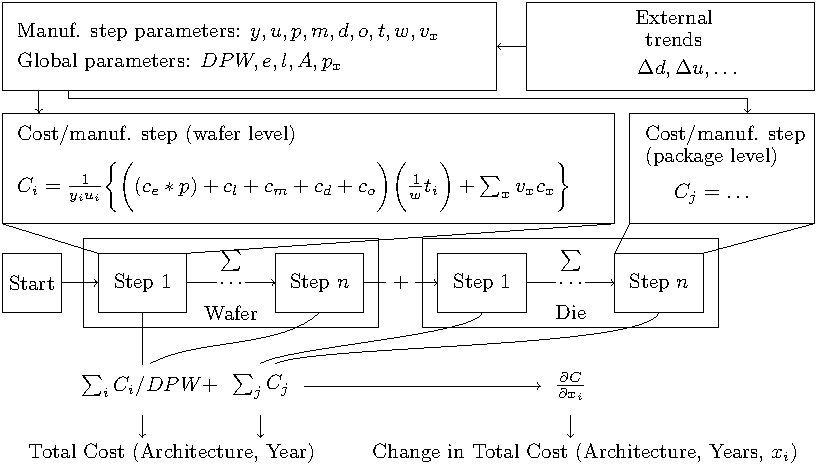
\includegraphics[width=0.95\textwidth]{./figures/cost_model.pdf}
    \caption{Schematic diagram of the cost model showing inputs to each step and computational steps leading to the cost model outputs. For the description of cost variables, see definitions for \cref{eqn:cost_wafer}. For the computation of total cost, see \cref{subsec:cost_computation}. For the computation of changes in total cost, see \cref{sec:contribution_variables}.}
    \label{fig:costmodel-schematic}
\end{figure}

The cost model adapted for this publication is a microeconomic manufacturing cost model. Within the timeframe and scope laid out in the main publication, it returns the total manufacturing cost of phosphor converted warm white light-emitting diode packages. In this computation, it considers the main economic factors associated with operating and maintaining manufacturing equipment. It does not consider costs associated with research and development or those associated with the construction of manufacturing facilities. It considers market trends through their effect on manufacturing parameters.

A schematic diagram of the cost model is presented in \cref{fig:costmodel-schematic}. The cost model is process step-based. It is split between the two stages of the manufacturing process: the first stage combining operations at the wafer level, followed by the LED packaging stage. The model takes as inputs parameters specific to individual manufacturing process steps (\textit{"manufacturing step parameters"}) and parameters affecting all manufacturing steps (\textit{"global parameters"}). The cost for each process step is then computed. The cost model returns returns the costs of individual manufacturing steps as well as the total manufacturing cost. It further considers the yield per step and returns the cumulative yield, the yielded cost per step and the yielded total manufacturing cost.

\subsubsection{Manufacturing Process Steps by Chip Architecture}

\cref{fig:manuf_classical_2003}-\cref{fig:manuf_csp_2020-2} show a simplified rendering of the manufacturing process of three different chip architectures considered in the cost model.

    %CLASSICAL CHIP

    \begin{landscape}
        \begin{figure}
            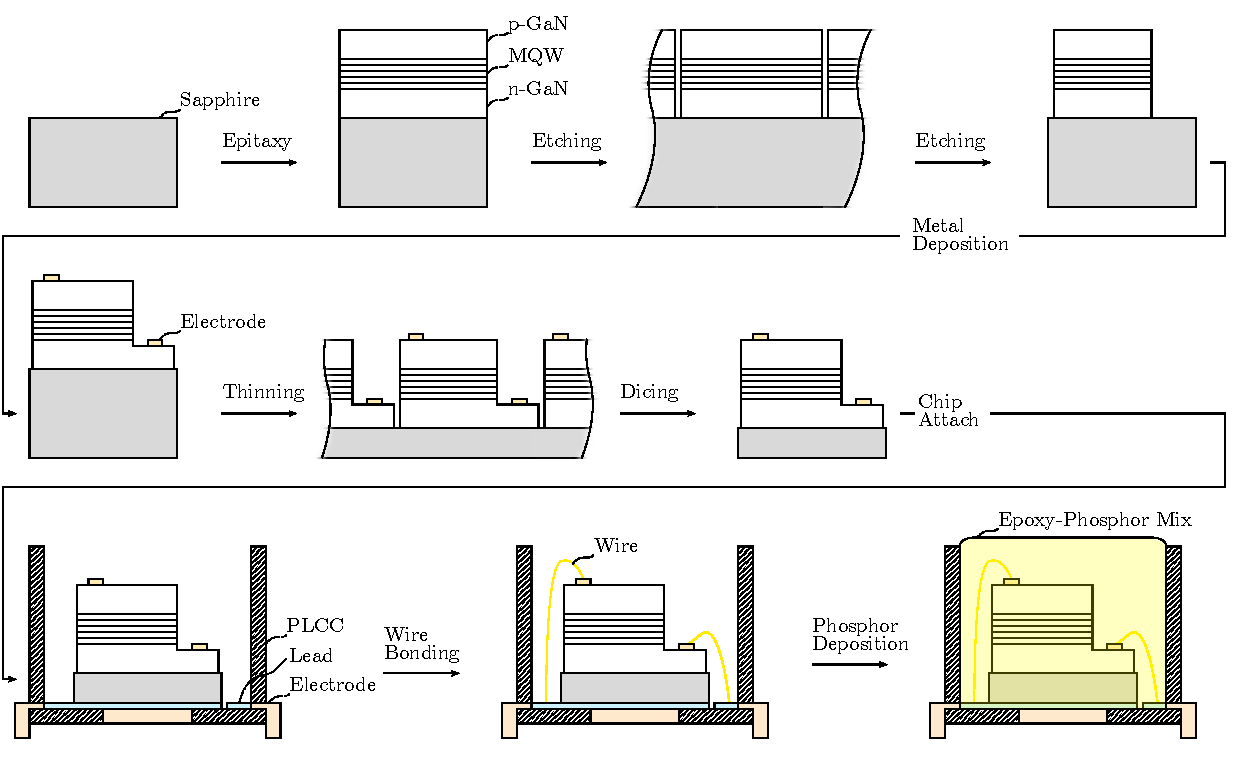
\includegraphics[width=555pt]{./figures/classical_overview_2003.pdf}
            \caption{Manufacturing process for a classical LED package with lateral current spreading, circa 2003. Abbreviations: MQW - multiple quantum well; PLLC - plastic leaded chip carrier.}
            \label{fig:manuf_classical_2003}
        \end{figure}
    \end{landscape}
    
    %VERTICAL THIN-FILM FLIP-CHIP

    \begin{landscape}
        \begin{figure}
            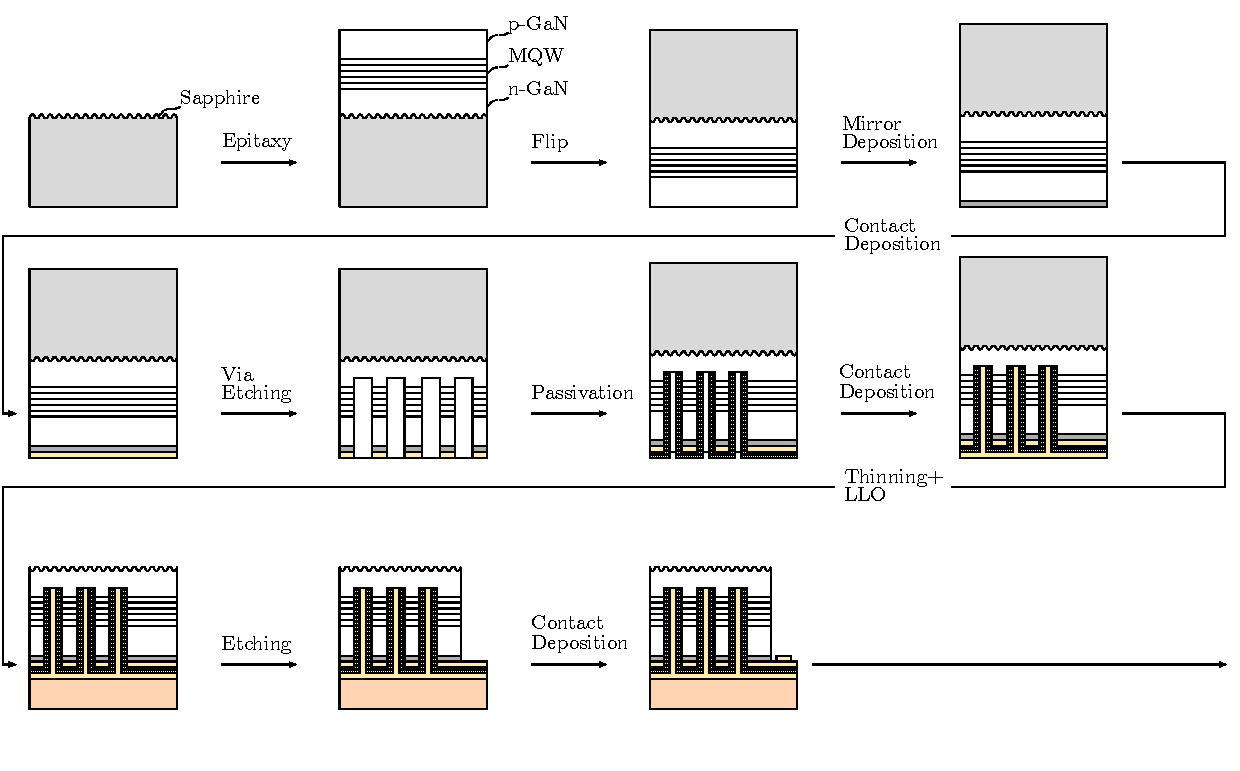
\includegraphics[width=595pt]{./figures/vtf_overview_2012-1.pdf}
            \caption{(1/2) Manufacturing process for a vertical thin-film  package flip-chip LED chip with vertical current spreading, circa 2012. Abbreviations: MQW - multiple quantum well; LLO - laser lift-off. Continued on next page.}
            \label{fig:manuf_vtf_2012-1}
        \end{figure}
    \end{landscape}

    \begin{landscape}
        \begin{figure}
            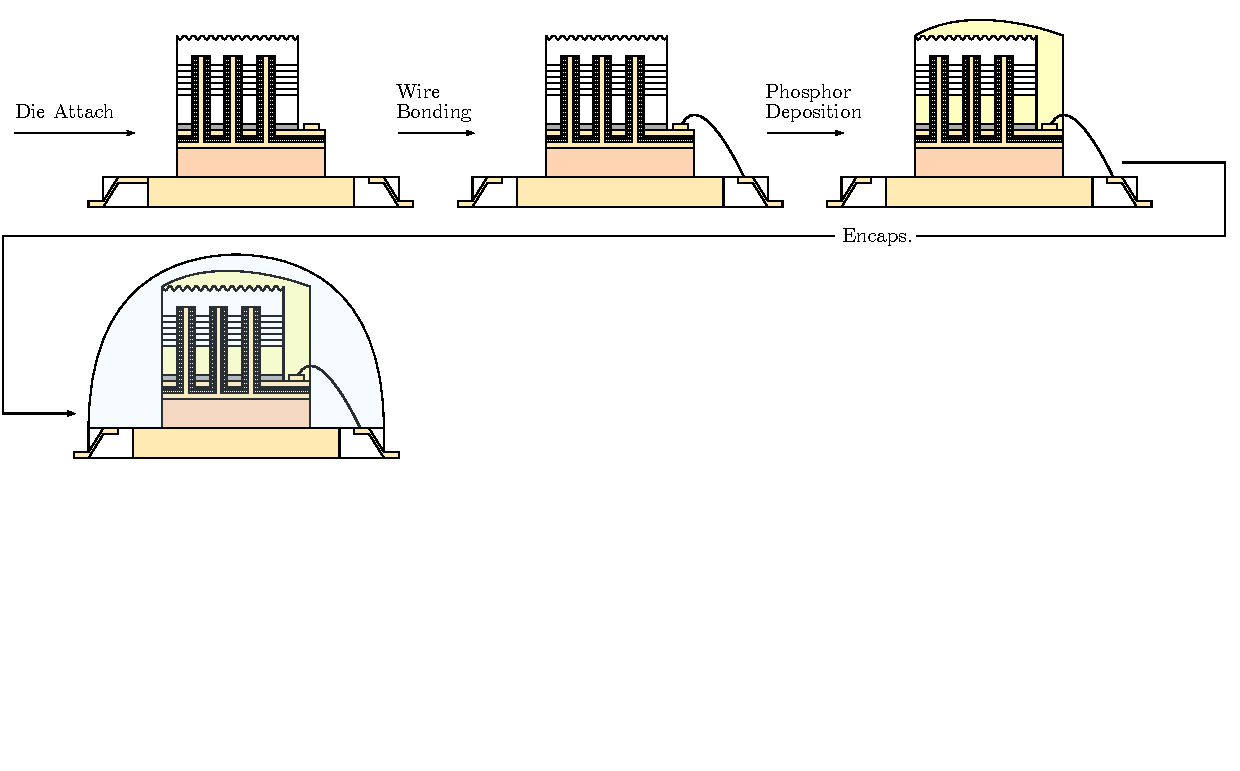
\includegraphics[width=595pt]{./figures/vtf_overview_2012-2.pdf}
            \caption{(2/2) Continued from previous page. Abbreviations: Encaps. - encapsulation.}
            \label{fig:manuf_vtf_2012-2}
        \end{figure}
    \end{landscape}

    % CHIP-SCALE PACKAGE FLIP-CHIP

    \begin{landscape}
        \begin{figure}
            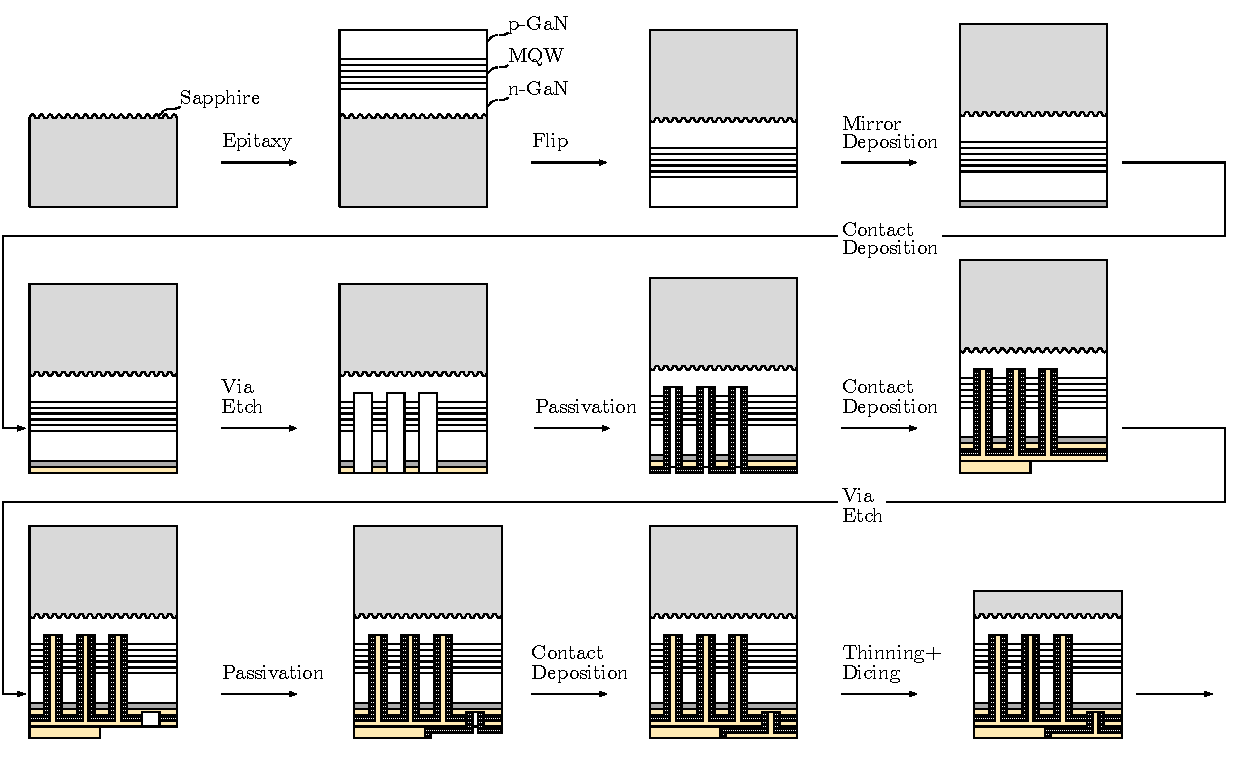
\includegraphics[width=595pt]{./figures/csp_overview_2020-1.pdf}
            \caption{(1/2) Manufacturing process for a chip scale package flip-chip LED chip with vertical current spreading, circa 2020. Abbreviations: MQW - multiple quantum well. Continued on next page.}
            \label{fig:manuf_csp_2020-1}
        \end{figure}
    \end{landscape}

    \begin{landscape}
        \begin{figure}
            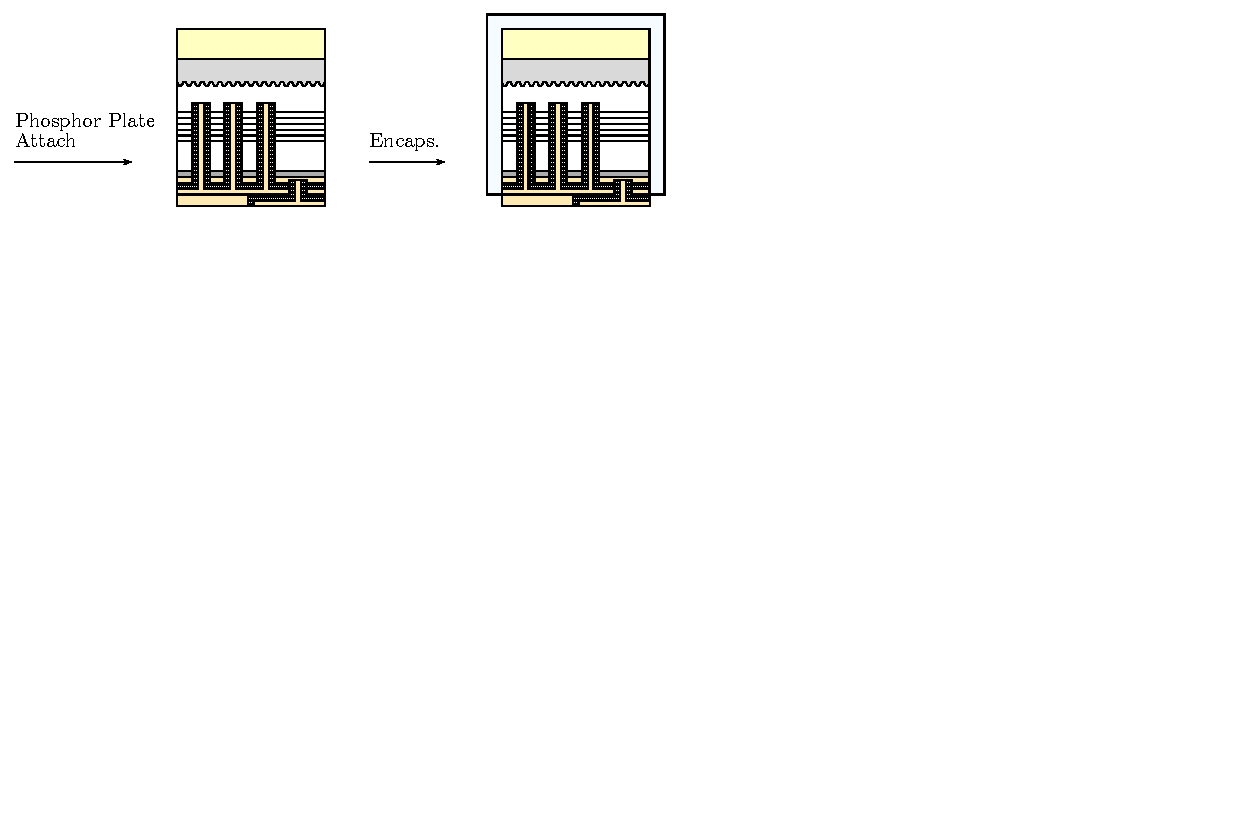
\includegraphics[width=595pt]{./figures/csp_overview_2020-2.pdf}
            \caption{(2/2) Manufacturing process for a chip scale package flip-chip LED chip with vertical current spreading, circa 2020. Continued from previous page. Abbreviations: Encaps. - encapsulation.}
            \label{fig:manuf_csp_2020-2}
        \end{figure}
    \end{landscape}

\subsubsection{Computation of Manufacturing Cost}
\label{subsec:cost_computation}

The manufacturing process of semiconductor devices can be categorized by the level at which manufacturing process steps are implemented, i.e., either at the wafer level or at the individual chip/package level. The total manufacturing cost per die is thus the sum of the total costs of all wafer processing steps and all die packaging steps.
\begin{equation}
\label{eqn:cost_sum}
    C \bigg[ \frac{ \text{USD}(2020) }{ \text{die} } \bigg] = P_S + C_w + C_p
\end{equation}
where
\begin{align*}
    P_S &\dots \text{sapphire substrate price per die} \\
    C_w &\dots \text{wafer processing cost per die} \\
    C_p &\dots \text{die processing cost}
\end{align*}
The total wafer processing cost and total die packaging costs are in turn the sum of all associated process steps.
\begin{equation}
        C_w = \sum_i C_i
\end{equation}
\begin{equation}
	C_p = \sum_j C_j
\end{equation}
The cost of a single process step $C_i$ can now be written as
\begin{equation}
\label{eqn:cost_wafer}
    C_i \bigg[ \frac{ \text{USD}(2020) }{ \text{die} } \bigg] =\frac{1}{DPW}  \frac{1}{y_i}   \bigg\{ \bigg((c_e*p) + c_l + c_m + c_d + c_o \bigg)_i \bigg( \frac{t_i}{w_i u_i} \bigg) + \sum_{x} v_x c_x \bigg\}
\end{equation}
where the index $i$ runs over all wafer processing steps, the index $j$ runs over all die processing steps and the index $x$ run over all materials.
\begin{align*}
        DPW &\dots \text{number of functional (i.e., successfully tested) die per wafer}\\
        y &\dots \text{process step yield} \\
        u &\dots \text{equipment utilization (relative to theoretical equipment capacity)} \\
        p &\dots \text{power consumption} \\
        c_e &\dots \text{hourly electricity cost} \\
        c_m &\dots \text{hourly maintenance cost} \\
        c_d &\dots \text{hourly depreciation cost}\\
        c_l &\dots \text{hourly labour cost} \\
        c_o &\dots \text{hourly overhead cost} \\
        t_i &\dots \text{time per run} \\
        w &\dots \text{wafers per run} \\
        A &\dots \text{wafer area} \\
        v_x &\dots \text{volume of material $x$ per wafer} \\
        c_x &\dots \text{cost of material $x$ per volume}\\
\end{align*}
The number of die per wafer $D$ depends on the total usable wafer area. The usable area depends on the wafer diameter, the cutting street width between the chips and the exclusion zone at the rim of the wafer.
\begin{equation}
	A_{\text{usable}}=A_{\text{wafer}}-A_{\text{cut}}-A_{\text{exclusion}}
\end{equation}
Determining the usable wafer area as a function of these three parameters requires a numerical solution. However, following discussions in the literature \cite{de2005investigation}, we approximate the number of functional die per wafer\footnote{often \textit{"good die per wafer"} in the literature} as
\begin{equation}
\label{eqn:dpw}
	DPW = \frac{\pi}{4}  \bigg ( \frac{d-2e}{\sqrt{a}+s/2} \bigg ) ^2 - \frac{\pi}{\sqrt{2}}\frac{d-2e}{(\sqrt{a}+s/2)^2}
\end{equation}
where
\begin{align*}
    d &\dots \text{wafer diameter} \\
    e &\dots \text{wafer edge exclusion zone width} \\
    a &\dots \text{die area} \\
    s &\dots \text{cutting street width} \\
\end{align*}

\begin{figure}[h!]
    \centering
    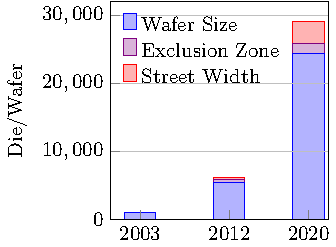
\includegraphics[width=5.5cm]{./figures/die-per-wafer.pdf}
    \caption{Number of die per wafer for the different wafer sizes used in different years: (DPW) $d(2002)=50$mm$\rightarrow851$DPW, $d(2002)=50$mm$\rightarrow5370$DPW, $d(2020)=100$mm$, \rightarrow26,838$DPW. Source: own estimates, based on \cref{eqn:dpw} and the dominant wafer size of the considered year, informed by expert interviews. For detailed statistics on changes in wafer size, compare also \cref{fig:wafers}.}
    \label{fig:dpw}
\end{figure}

Results are plotted in \cref{fig:dpw}, showing the increase in die per wafer (DPW) over time. \cref{eqn:dpw} then gives us for the cost of a manufacturing step $C_i$ in the wafer processing category
\begin{equation}
\label{eqn:cost_wafer_full}
\begin{split}
    C_i \bigg[ \frac{ \text{USD}(2020) }{ \text{die} } \bigg] &= \bigg (  \frac{\pi}{4}  \bigg ( \frac{d-2e}{\sqrt{a}+s/2} \bigg ) ^2 - \frac{\pi}{\sqrt{2}}\frac{d-2e}{(\sqrt{a}+s/2)^2} \bigg )^{-1} \times \\
    &  \frac{1}{y_i}  \bigg\{ \bigg((c_e*p) + c_l + c_m + c_d + c_o \bigg)_i \bigg( \frac{t_i}{w_i u_i} \bigg) + \sum_{x} v_x c_x \bigg\}
\end{split}
\end{equation}
and the cost of a manufacturing step $C_j$ in the packaging category
\begin{equation}
\label{eqn:cost_die}
    C_j \bigg[ \frac{ \text{USD}(2020) }{ \text{die} } \bigg] = \frac{1}{y_j}  \bigg\{ \bigg((c_e*p) + c_l + c_m + c_d + c_o \bigg)_i  \frac{c_j}{u_j} + \sum_{x} a v_x c_x \bigg\}
\end{equation}
where $c_j$ is $\text{throughput}^{-1}$. The total cost is thus
\begin{equation}
\label{eqn:cost_total}
\begin{split}
    C= P_s &+ \sum_i \bigg \{ \frac{1}{DPW} \frac{1}{y_i} \bigg[ \frac{t_i}{w_i u_i} \bigg((e*p) + l + m + d +o \bigg)_i  + \sum_{x} v_x p_x \bigg] \bigg \} + \\
    & + \sum_j \bigg \{ \frac{1}{y_j} \bigg[ \frac{c_j}{u_j}  \bigg((e*p) + l + m + d + o \bigg)_i + \sum_{x} a v_x p_x \bigg ] \bigg\}
\end{split}
\end{equation}
Note that in keeping with the categorization introduced by the United States Department of Energy (cf. eg. \cite{doe_ssl_rnd_2019}), certain steps from these two categories are reported separately. In the wafer processing category, the epitaxy step is reported separately due to its complexity and the large share of cost carried. In the wafer processing category, the phosphor step is reported separately.

\subsubsection{Computation of Yielded Cost}

Devices may be damaged or otherwise rendered unusable during the manufacturing process. The ratio between the number of good devices per step and the number of handled devices per step is known as the yield. Optimizing this yield is critical for reducing manufacturing cost \cite{Kumar2006}. This is because cumulative yield quickly drops as the yield from manufacturing steps with below 100\% yield is multiplied. We must thus consider not only the manufacturing cost per process step, but also the cost including the yield \cite{becker2001use}\cite{becker2001using}. While there are different mathematical approaches to including yield, we follow the definition in \cite{becker2001use}. We write for the yielded cost $C_{Y_i}$ of a step $i$ with associated cost (before considering yield) $C_1$ and yield $Y_1$:

\begin{equation}
\label{eqn:C_2}
    C_{Y_1} = \frac{C_1}{Y_1}
\end{equation}
\begin{equation}
    C_{Y_2} = \frac{C_1 + C_2}{Y_1 Y_2} - C_{Y_1} = \frac{C_1 + C_2}{Y_1 Y_2} - \frac{C_1}{Y_1} = \frac{1}{Y_1 Y_2} \bigg ( C_1 (1-Y_2) +C_2 \bigg)
\end{equation}
\begin{equation}
    C_{Y_i} = \frac{ \sum_{x \leq i} C_x }{ \prod_{x \leq i} Y_x } - \frac{ \sum_{x<i} C_x }{ \prod_{x<i} Y_x }
\end{equation}

If a step is applied more than once, we can conveniently rewrite this in a form suited to computation within the \textit{Excel} worksheet. Assuming step $2$ is used twice, we get for the yielded cost of this step an equation of the form

\begin{equation}
\label{eqn:C_2^2}
    C_{Y_2}^{(2 \times)} = \bigg( \frac{C_1 + C_2}{Y_1 Y_2} - \frac{C_1}{Y_1} \bigg) + \bigg( \frac{C_1 + 2 C_2}{Y_1 Y_2^2} - \frac{C_1 + C_2}{Y_1 Y_2}     \bigg)
\end{equation}
\begin{equation}
    = \frac{1}{Y_1 Y_2^2} \bigg( C_1 (1-Y_2^2) +2C_2 \bigg)
\end{equation}

which can be compared to  \cref{eqn:C_2} to find a more general form:

\begin{equation}
    C_{Y_2}^{(n \times)} = \frac{1}{Y_1 Y_2^n} \bigg( C_1 (1-Y_2^n)+nC_2\bigg)
\end{equation}

It can be shown by induction that the general form of a term for a step $i>1$ repeated $n$ times can be expressed as:

\begin{equation}
\label{eqn:yielded_cost}
    C_{Y_{i>1}}^{(n \times)} = \frac{1}{Y_i^{n-1} \prod_{x \leq i} Y_x} \bigg( nC_i + \sum_{x < i} C_x (1-Y_i^n) \bigg)
\end{equation}

This cumulative approach to yielded cost is different from the approach taken in the original \textit{LEDCOM} model. It uses what in the literature is described as an \textit{"itemized approach"} to yielded cost \cite{becker2001use}. In this approach, the yielded cost of a single process step $f$ is described as

\begin{equation}
    f_\text{single} = \frac{i+s}{y}
\end{equation}

where

\begin{align*}
    i &\dots \text{material cost of previous step} \\
    s &\dots \text{step cost}
\end{align*}

For process steps that are performed more than once, a series expression is used

\begin{equation}
    f_{\times 2} =  \frac{\frac{i+s}{y}+s}{y}
\end{equation}
\begin{equation}
\label{eqn:series}
    f_{\times n} = \frac{i + s(1+y+y^2+ \dots + y^{n-1})}{y^n}
\end{equation}

This itemized approach serves as a convenient approximation, but its cumulative contributions do not equal the total yielded cost of the entire manufacturing process

\begin{equation}
    f_\text{total} = \frac{\sum_i^n s_i}{\prod_i^ny_i} \neq \sum_i^n f_i
\end{equation}

where $n$ is the total number of steps. This is due to the approximation introduced through the series approximation in  \cref{eqn:series}.

\subsubsection{Example of Input Data Considered: Sapphire Wafers}

Sapphire wafers form the substrate on which all other layers of the light-emitting diode are grown. Being transparent to radiation in the visible spectrum, it is not removed after growth in the Classical architecture or the Thin-Film Flip-Chip architecture. In the Vertical Thin-Film architecture, it is removed by means of a laser-lift-off process. Wafers can be either unpatterned or patterned, where the latter has become commonplace by 2020 due to the beneficial properties that microstructures on the surface have on layer growth \cite{wuu2009defect} and light-extraction efficiency \cite{lee2006enhancing}. The price of sapphire substrates has decreased significantly since the year 2000, as shown in the bottom panel of \cref{fig:wafers}. This can be attributed not only to the lighting industry, but more importantly to increased supply as a result of increased demand from electronics manufacturing \cite{yole2015sapphire}, where sapphire glass is used to protect screens and sensor interfaces from scratches \cite{khattak2016world}. Wafer sizes used in manufacturing have also increased, due to the favourable economics of large wafer processing. The market has been dominated by U.S.-based \textit{Rubicon Technology} and Russian-based \textit{Monocrystal}. The evolution of sapphire wafer prices and diameters used in LED manufacturing over the years is shown in top panel of \cref{fig:wafers}.

\begin{figure}[h!]
    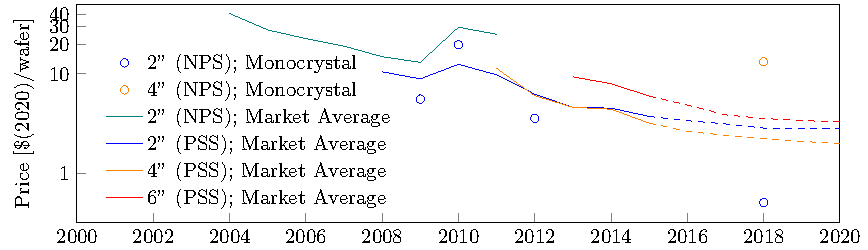
\includegraphics[width=15cm]{./figures/sapphire_prices.pdf}
    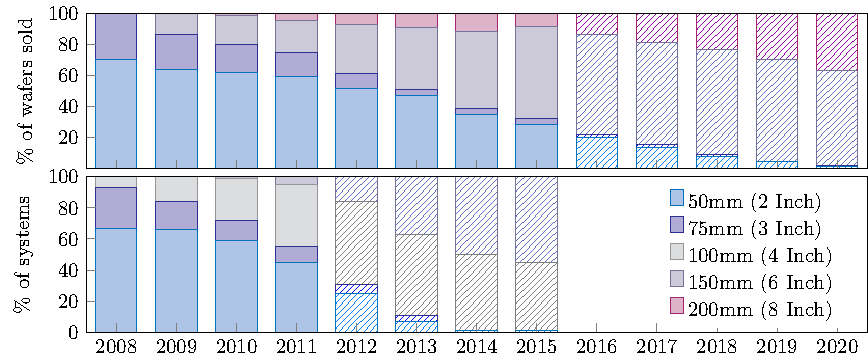
\includegraphics[width=14.5cm]{./figures/wafer_size.pdf}
	\caption{Top: Historical data for sapphire substrate prices of different surface properties and diameters. Shown is data for polished surface (NPS) and patterned substrates (PSS). \textit{Monocrystal} denotes the Russian manufacturer of the same name. Dashed lines are projections from the previous year. Sources: \cite{monocrystal2020private}\cite{yole2011sapphire}\cite{yole2015sapphire}. Bottom: Prevalence of sapphire wafer size used in the manufacturing of light-emitting diodes. Hatched bars are projections given by the sources. Sources: \cite{veeco2013}\cite{Scholand2012}\cite{yole2015sapphire}}
	\label{fig:wafers}
\end{figure}

\newpage
\subsubsection{Preliminary Sensitivity Analysis}

\begin{figure}[]
	\centering
    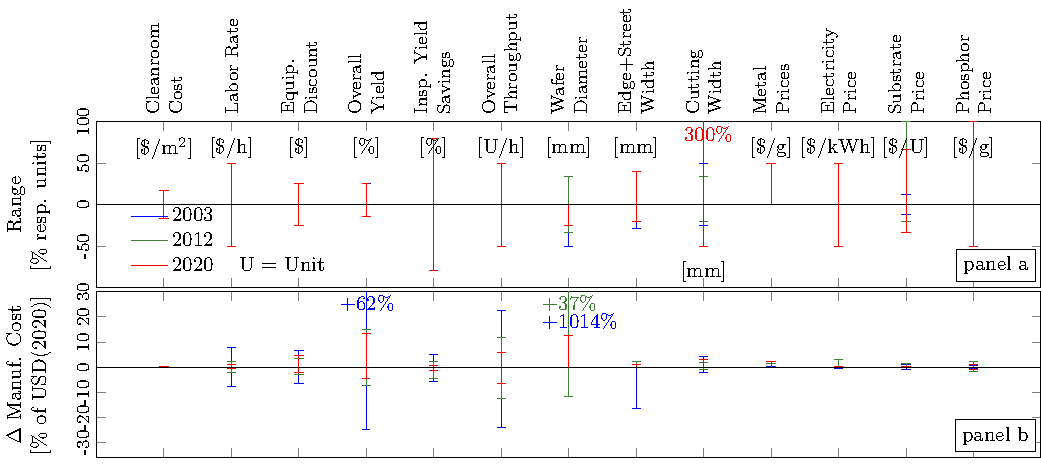
\includegraphics[width=\textwidth]{./figures/costmodel_sensitivity.pdf}
	\caption{Sensitivity analysis for selected cost model parameters. Panel a represents the tested range of variation of parameters indicated on horizontal axis along with their respective measurement units, as represented in \cref{tab:sensitivity}. Panel b shows the resulting range of variation in the manufacturing cost. Ranges are represented for three years considered in the cost model, where corresponding data is available, by whiskers of the following colour: 2003 – blue, 2012 – green, 2020 – red. Note the overall trend of decreasing sensitivity to cost model parameters as the number of die per wafer increases over time. Abbreviations: resp. - respective; yield sav. from insp. - yield savings from inspection.}
	\label{fig:sensitivity}
\end{figure}

A sensitivity analysis of the cost model has been performed using parameter variations listed in table \cref{tab:sensitivity}. The amount of parameter variation was chosen to encompass the identified range of parameter values in different manufacturing setups for each considered year. As an example, the lower range in the variation for the price of metals used in the model (+50\%,-0\%) was chosen because the prices quotes from the United State Geological Survey price database. Industry metals are not sold below the price of the raw material and often the markup is small compared to the price of the material. The upper range was chosen because a survey of industrial metal suppliers for semiconductor manufacturing showed that the largest markup was below 50\%. The results of the analysis are shown in  \cref{fig:sensitivity}. The cost model is generally more sensitive to the variation in parameters at smaller wafer diameters. The most sensitive parameters are global parameters, such as yield or average equipment throughput.

\begin{table}[]
\small
    \caption{Cost model sensitivity analysis parameter list. The results of the sensitivity analysis for the parameters in this table are presented in \cref{fig:sensitivity}.}
    \vspace{5mm}
    \begin{NiceTabularX}{\textwidth}{ |X|X|l|l|l|l|l|l|X|}
        \hline
            \textit{Parameter} & \textit{Unit} & \textit{2003} & $\pm [\%]$ & \textit{2012} & $\pm [\%]$ & \textit{2020} & $\pm [\%]$ & Source \\
        \hline
            Cleanroom Cost & \text{USD}/m$^2$ & 3000 & +16,-16 & 3000 & +16,-16 & 3000 & +16,-16 & \cite{mddi1997cleanroom}\cite{ledcomv2} \newline \cite{bakshi2009euv}\cite{gajera2006process} \\
        \hline
            Person-hour & FTE & 100\% & +50,-50 & 100\% & +50,-50 & 100\% & +50,-50 & I \\
        \hline
            Equip. Discount & \% of \text{USD} & 0\% & +25,-25 & 0\% & +25,-25 & 0\% & +25,-25 & I \newline \cite{Appleyard_2001} \\
        \hline
            Overall Yield & \% & 100\% & +25,-25 & 100\% & +25,-15 & 100\% & +25,-25 & I, \cite{lumi2012yield}\cite{ledsmag2012} \newline \cite{systemplus2015reverse}\cite{ledcomv2} \\
        \hline
            Inspec. Yield Savings & \%/inspec. & 0.5\% & +80,-80 & 0.5\% & +80,-80 & 0.5\% & +80,-80 & \cite{mckinseyyield} \\
        \hline
            Overall Throughput & UPH or h$^{-1}$ & 100\% & +50,-50 & 100\% & +50,-50 & 100\% & +50,-50 & Datasheets \\
        \hline
            Wafer Diameter & mm & 100 & +0,-50 & 150 & +33.3,-33.3 & 200 & +0,-25 & I and \cref{fig:wafers} \\
        \hline
            Edge Exclusion & mm & 7 & +0,-50 & 5 & +40,-0 & 5 & +40,-20 & \cite{ledsmagexclusion}\cite{rubiconexclusion} \newline \cite{xiamenexclusion}\cite{american2007annual} \\
        \hline
            Cutting Width & $\mu$m & 100 & +50,-25 & 75 & +33.3,-20 & 20 & +300,-50 & \cite{masaki2000division}\cite{ils2005width} \newline \cite{photonics2010width}\cite{discowidth} \\
        \hline
            Metal Prices & \text{USD}/kg & 100\% & +50,-0 & 100\% & +50,-0 & 100\% & +50,-0 & Datasheets \\
        \hline
            Electricity Price & \text{USD}/kWh & 100\% & +50,-50 & 100\% & +50,-50 & 100\% & +50,-50 & \cite{eia2000electric}\cite{eia2019electric} \\
        \hline
            Saph. Subst. Price & \text{USD} & 40 & +12.5,-12.5 & 10 & +100,-20 & 3 & +66.6,-33.3 & \cref{fig:wafers} \\
        \hline
            Phosphor Prices & \text{USD}/g & 100\% & +50,-50 & 150 & +0,-0 & 200 & +0,-0 & I, \cite{yole_phosphor_2012}\cite{yole2017phosphor} \\
        \hline
        \end{NiceTabularX}
    \vspace{5mm}
    
    Note: The units for the values in columns \textit{2003}-\textit{2020} are indicated in the column \textit{Units}. If values in columns \textit{2003}-\textit{2020} are instead given in \%, this indicates that the parameters were varied by a set percentage from their respective model baselines. Abbreviations: FTE - full-time equivalent; UPH - units per hour; Equip. Discount - equipment discount (sales rebate for large purchases); Inspec. Yield Savings - yield savings from inspection (early detection and alleviation of issues in the manufacturing workflow).
    \label{tab:sensitivity}
\end{table}

\newpage
\subsection{Computation of Contribution of Individual Variables}
\label{sec:contribution_variables}

To quantify the drivers of changes in manufacturing cost or device performance among many contributing factors, one would need to identify the magnitude of contribution to these changes made by single variables in equations \cref{eqn:cost_wafer} and \cref{eqn:cost_die}. Mathematically, given a function $C$ which describes the manufacturing cost or performance function of a device at time $t$,
\begin{equation}
F=ab+cd
\end{equation}
and input variables $a,b,c,d$, we are looking for the contribution $\Delta F_{a}$ made by a single variable $a$ to the total change in the function value $\Delta F$ between points $t_0,t_1$ such, that
\begin{equation}
\Delta F = F(t_1)-C(t_0) = \sum_{i=a, \dots, d} \Delta F_i
\end{equation}
The infinitesimal contribution to the total funcation value by the infinitesimal change in an input variable is defined through the total differential of the function as
\begin{equation}
\text{d}F(x_1 (t), x_2(t), \dots) = \sum_i \frac{\partial F }{\partial x_i}     \frac{\text{d}x_i}{\text{d}t} = \sum_i \frac{\partial F }{\partial x_i}  \Delta x_i
\end{equation}
where $x_i$ is an input cost variable. The contribution of the change $\Delta x_1$ in variable $x_1$ to the total function value $F$ over the period $t_0 < t < t_1 $ is then
\begin{equation}
\Delta F_{x_1} = \int_{t=t_1}^{t_2} \frac{\partial F }{\partial x_1} \frac{\text{d}x_1}{\text{d}t} \text{d}t
\label{eqn:integral_1}
\end{equation}
However, data on the input variables is not available in continuous time. Disaggregating the contribution of single variables to the change in the cost or performance is thus not straightforward in our model. This problem does not arise in cost models which compute cost changes directly, such as \cite{nemet2012solar} \cite{goodrich2013assessing}. In our work, we propose to address this problem by following an approach developed by Kavlak et al. \cite{kavlak2018evaluating}. For the detailed derivation, we refer to this publication.

The function $F$ as a function of a vector of input model variables $\vec{r}=(r_1,r_2,\dots)$ is defined as
\begin{equation}
    F(\vec{r}) = F(r_1,r_2, \dots) = \sum_i F_i
\end{equation}
where
\begin{equation}
    F_i(\vec{r}) = F_i^0 \prod_w g_{iw}(r_w)
\end{equation}
Using logarithmic differentiation, the integral from  \cref{eqn:integral_1} can be rewritten as
\begin{equation}
    \Delta F_x = \int_{t=t_0}^{t_1} F(t) \frac{ \partial \ln F }{ \partial x } \frac{ \text{d} x }{ \text{d} t} \text{d} t
\end{equation}
where for $F(t)$ a constant $F(t) \approx \tilde{F} $ can be chosen such that $\Delta F_{x_i} = \Delta F$. In practice, this constant value can be approximated through the geometric and arithmetic means $\tilde{F} \approx \frac{2}{3} F_i^\text{geo} + \frac{1}{3} \overline{F_i}$. The contribution of a single cost model variable $r_z$ can then be written as
\begin{equation}
    \Delta F_z (t_1,t_2) \approx \sum_i \tilde{F_i} \ln \frac{g_{iz}(t_2)}{g_{iz}(t_1)}
\end{equation}
We use this approach to estimate the effect of individual innovations and spillovers on LED device performance, as discussed in section 4.3 and shown in Figure 5 in the main article. Due to time constraints, we leave the quantification of the impact of different drivers of cost reductions with this methodological approach for our future work.


\end{document}